\section{相关技术}

\subsection{Hadoop}

\begin{frame}[t]{相关技术(Hadoop)}
    \textbf{Hadoop}是Apache基金会推出的大数据计算平台,其中HDFS(Hadoop Distributed File System)
    是Hadoop数据存储基础

    \pause
    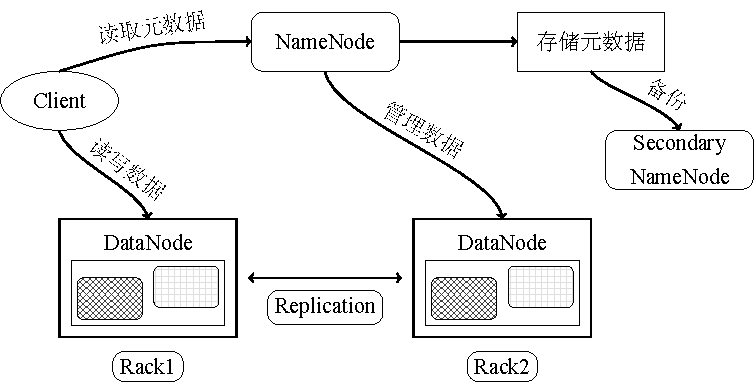
\includegraphics[scale=0.8]{figures/hdfs.pdf}
\end{frame}

\begin{frame}[t]{相关技术(Hadoop)}
    \textbf{Hadoop MapReduce}是Hadoop平台的计算框架,开发人员只需要关注Map函数和Reduce函数就可
    以实现分布式计算

    \pause
    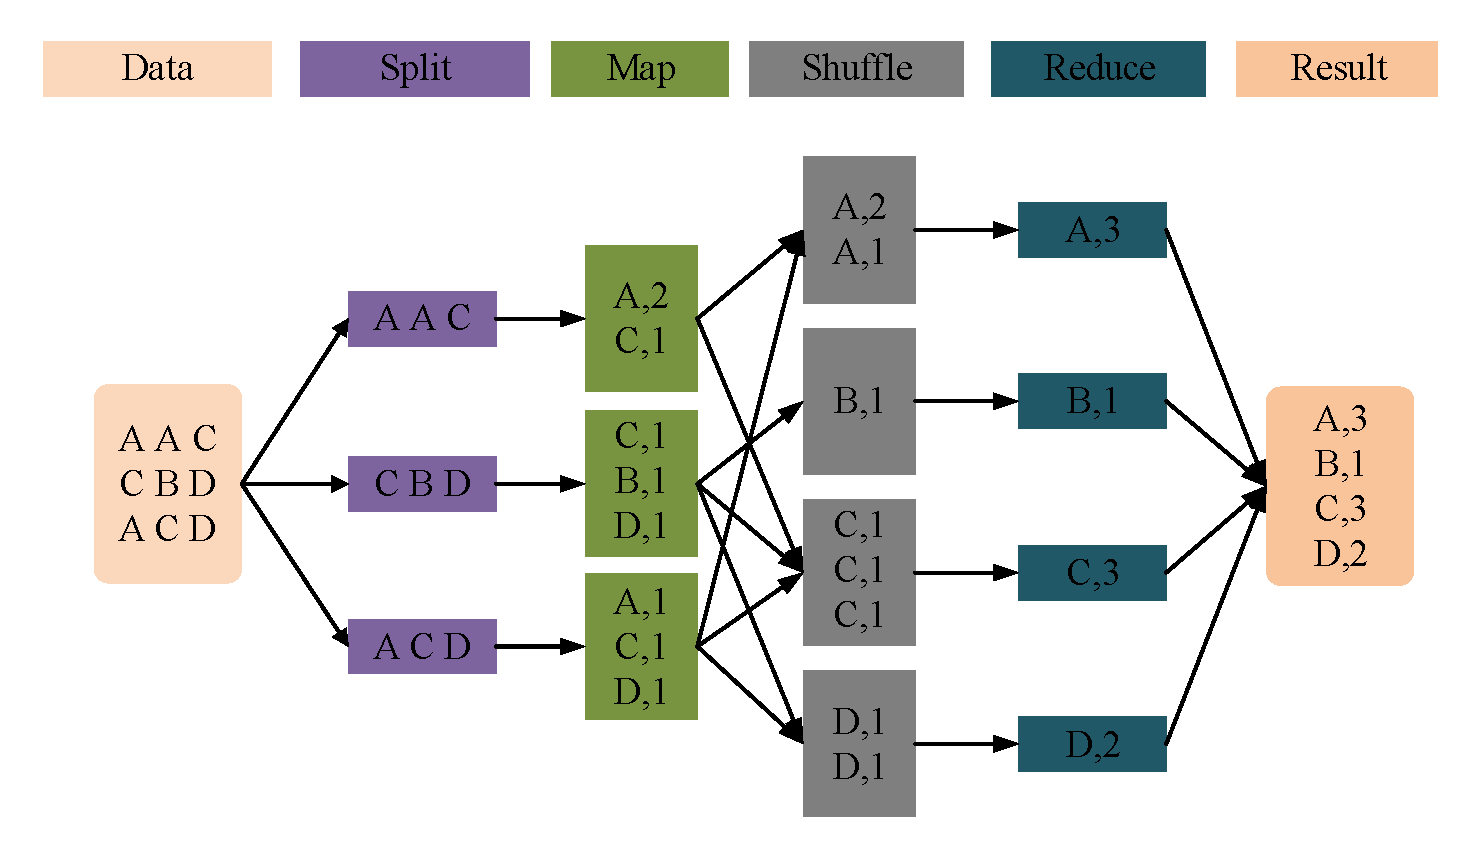
\includegraphics[scale=0.4]{figures/mapreduce.pdf}

    \pause
    \alert{缺陷: }单点故障、算子抽象、IO操作频繁
\end{frame}

\subsection{Spark}

\begin{frame}[c]{相关技术(Spark)}
    \begin{columns}
        % one column
        \begin{column}{0.5 \textwidth}
            \textbf{Spark}是AMP实验室打造的开源的并行计算框架,拥有完整的技术生态系统。

            \vspace{0.5em}
            \begin{figure}
                \centering
                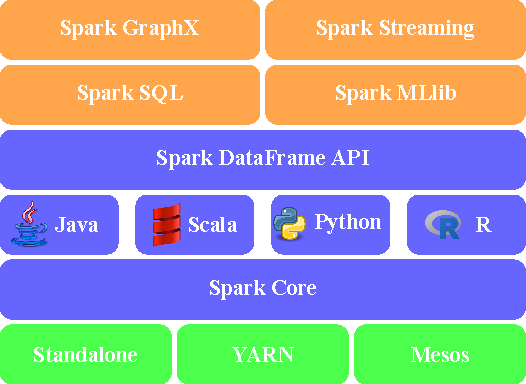
\includegraphics[scale=0.6]{figures/spark.pdf}
            \end{figure}            
        \end{column}

        %next column
        
        \pause
        \begin{column}{0.5 \textwidth}
            \begin{itemize}
                \item \textbf{Spark SQL}: 类SQL语言查询结构化数据
                \item \textbf{Spark MLlib}: 常用机器学习算法Spark实现
                \item \textbf{Spark GraphX}: 分布式图及其计算Spark实现
                \item \textbf{Spark Streaming}: Spark流应用计算框架
            \end{itemize}
        \end{column}
    \end{columns}
\end{frame}

\begin{frame}[c]{相关技术(Spark)}
    弹性分布式数据集(RDD)是Spark的核心抽象,在内存中已被分区、只读的、并提供
    一组丰富的操作方式的数据\textbf{集合}。RDD选择血统机制来提高系统的容错性,
    一旦数据出错,通过血统可以迅速恢复。

    \vspace{0.5em}
    \pause
    RDD提供了丰富的接口来操作数据集合,主要分为两种:
    \begin{itemize}
        \item \textbf{Transformation:} 可以理解为认为分配的过程,返回值仍然是一个RDD,采用Lazy策略
        \item \textbf{Action:} 将RDD持久化起来,将Tansformation的分配的操作执行
    \end{itemize}

\end{frame}

\begin{frame}[c]{相关技术(Spark)}
    \begin{columns}
        \begin{column}{0.5 \textwidth}
            Spark一栈式解决方案的\alert{优势:}
            
            \vspace{0.5em}
            \begin{itemize}
                \item 快速处理,内存计算
                \item 通用性,技术方案无缝集成
                \item 与Hadoop集群集成
            \end{itemize}
        \end{column}

        \pause
        \begin{column}{0.5 \textwidth}
            Spark在处理海量空间数据\alert{劣势:}

            \vspace{0.5em}
            \begin{itemize}
                \item 不支持空间数据类型
                \item 不支持空间操作
                \item 没有空间数据优化
            \end{itemize}
        \end{column}
    \end{columns}

\end{frame}

\subsection{微博数据接口}

\begin{frame}[c]{微博数据接口}
    新浪微博提供了API方便第三方程序访问微博丰富的数据资源

    \begin{figure}
        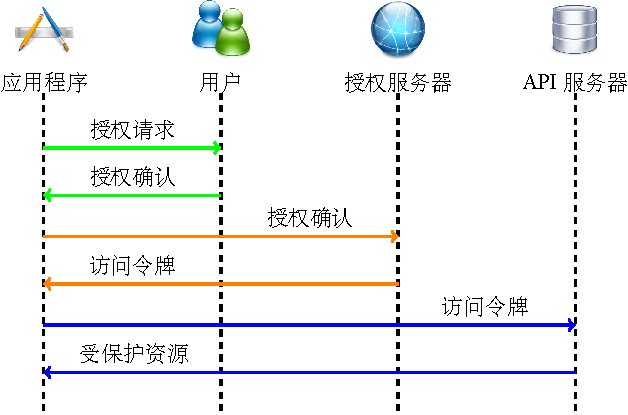
\includegraphics[scale=0.8]{figures/api.pdf}
    \end{figure}
\end{frame}

\begin{frame}[c,c]{微博数据接口}
    微博API接口实际上是一系列HTTP GET请求,返回微博用户上传的数据,其中包含了
    用户位置数据。

    \vspace{0.5em}
    \pause
    \begin{itemize}
    \item location/geo/address\_to\_geo $\rightarrow$  根据地址返回地理信息坐标 
    \item location/pois/show\_batc $\rightarrow$ 批量获取POI点的信息
    \item location/citycode $\rightarrow$ 城市代码对应表
    \item place/nearby/pois $\rightarrow$ 获取附近的POI点
    \end{itemize}
\end{frame}

